%%%%%%%%%%%%%%%%%%%%%%%%%%%%%%%%%%%%%%%%%%%%%%%%%%%%%%%%%%%%%%%%%%%%%%%%%%%%%%%%%%%%%%%%%%%%%%%%%%%%%%%%%%%%%%%%%%%%%%%%%%%%%%%%%%%%%%%%%%%%%%%%%%%%%%%%%%%%%%%%%%%%%%%%%%%%%%

\UC{Inserimento nuovo indirizzo di consegna}
\label{inserimento-indirizzo-consegna}

\begin{figure}[H]
    \centering
    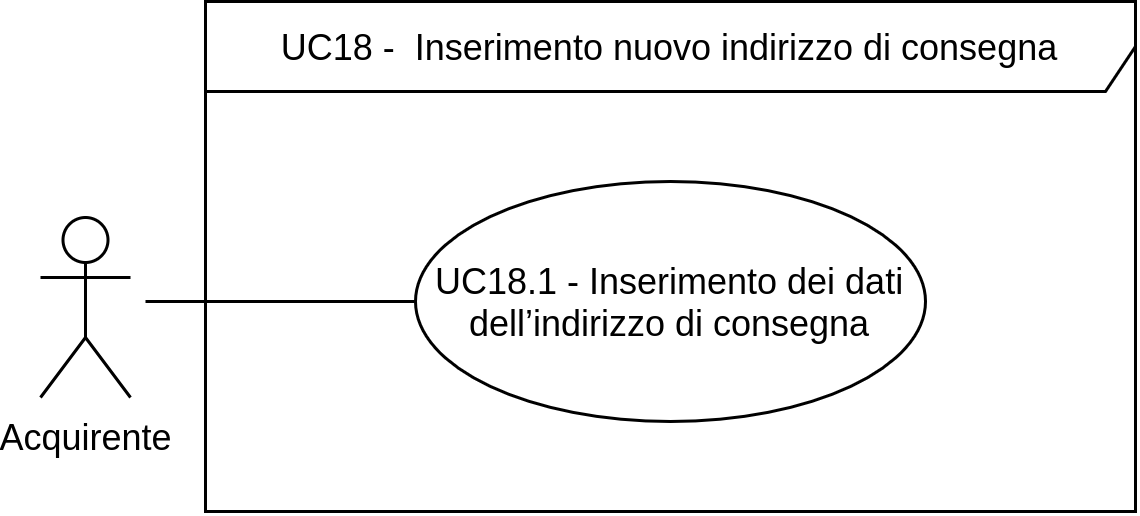
\includegraphics[scale=1]{Immagini/DiagrammiUC/Acquirente/InserimentoIndirizzoConsegna.png}
    \caption{Diagramma di \actualUC: Inserimento nuovo indirizzo di consegna} 
    \label{fig:inserimento-indirizzo-consegna}
\end{figure}

L'acquirente vuole aggiungere un nuovo indirizzo di consegna.
\begin{itemize}
    \item \textbf{Attori primari:} acquirente;
    \item \textbf{Precondizione:} l'acquirente è nell'operazione di checkout e ha selezionato la funzione di aggiunta di un nuovo indirizzo per la consegna;
    \item \textbf{Postcondizione:} l'acquirente ha inserito il nuovo indirizzo di consegna;
    \item \textbf{Scenario principale:} l'acquirente è nell'operazione di checkout e vuole inserire un nuovo indirizzo di consegna. Per poterlo fare dovrà premere sull'azione di aggiunta nuovo indirizzo ed eseguire le seguenti azioni:
    \begin{itemize}
        \item (UC\ref{inserimento-indirizzo-consegna.modulo}) - Inserimento dei dati dell'indirizzo di consegna; 
        \item Confermare l'aggiunta del nuovo indirizzo di consegna.
    \end{itemize}
    \item \textbf{Scenari alternativi:}
    \begin{enumerate}[label=\lett]
        \item Se non viene confermata l'aggiunta del nuovo indirizzo di consegna, allora non verrà aggiunto e si andranno a perdere tutti i dati relativi ad esso che sono stati inseriti.
    \end{enumerate}
\end{itemize}

\subUC{Inserimento dei dati dell'indirizzo di consegna}
\label{inserimento-indirizzo-consegna.modulo}

\begin{figure}[H]
    \centering
    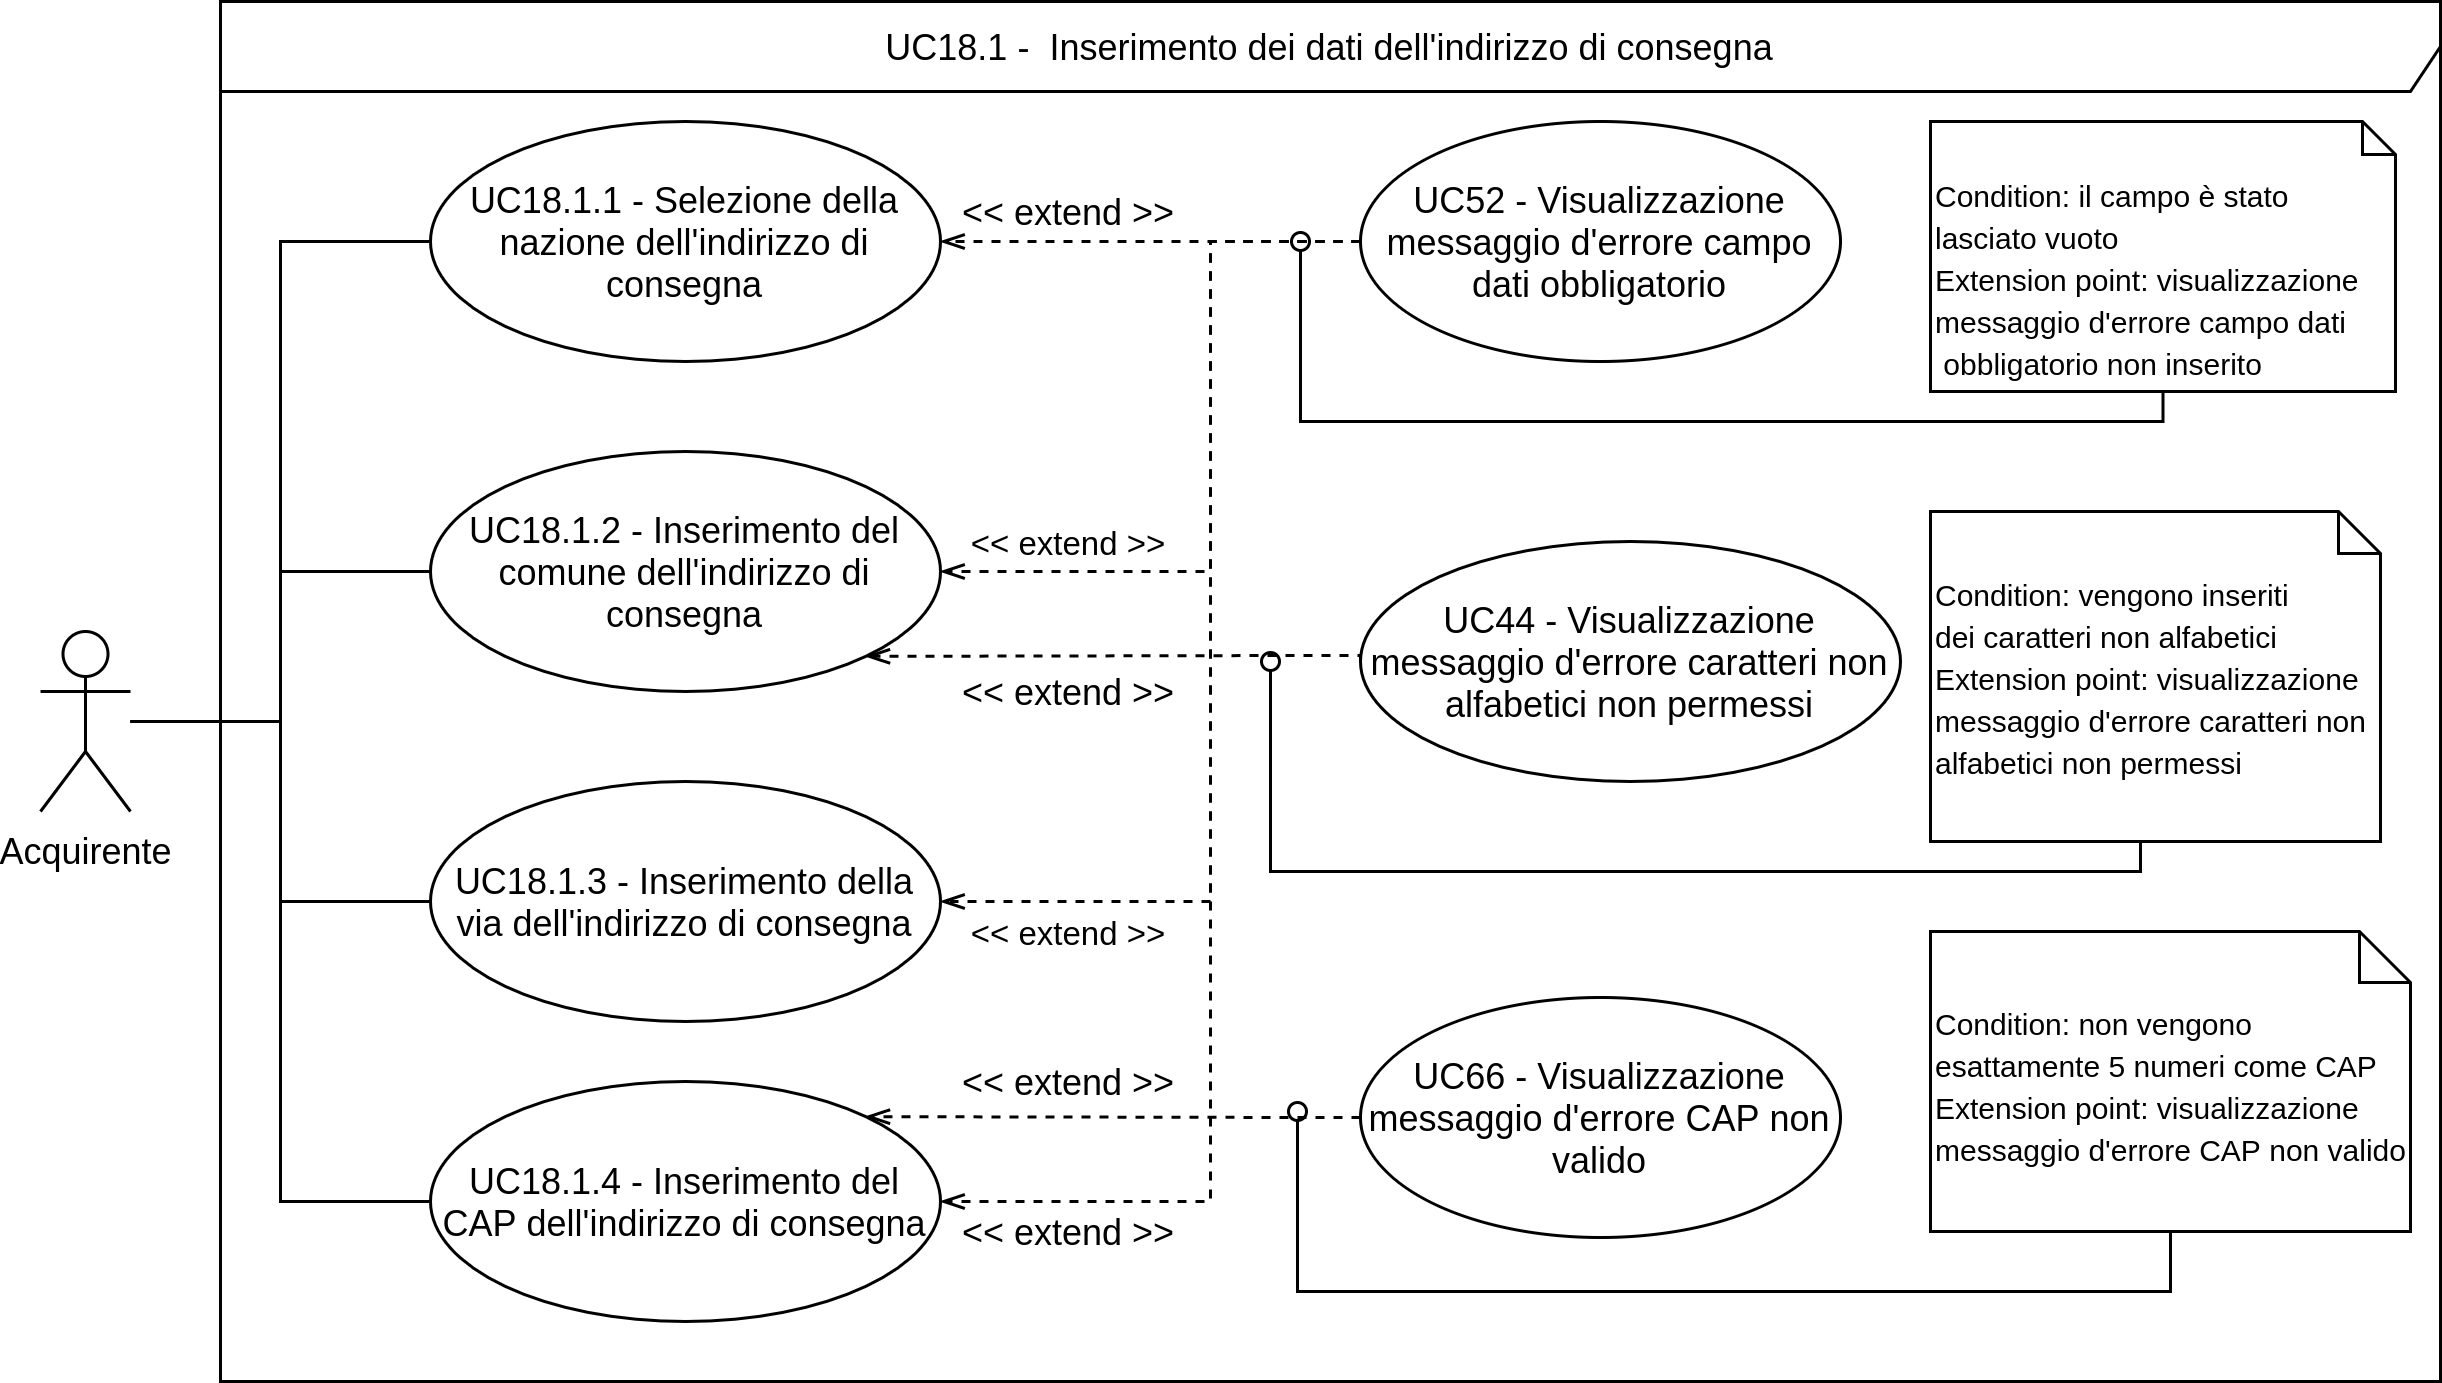
\includegraphics[scale=0.6]{Immagini/DiagrammiUC/Acquirente/InserimentoDatiIndirizzoConsegna.png}
    \caption{Diagramma di \actualSubUC: Inserimento dei dati dell'indirizzo di consegna} 
    \label{fig:inserimento-indirizzo-consegna.modulo}
\end{figure}

L'acquirente compila il modulo per aggiungere un nuovo indirizzo di consegna.
\begin{itemize}
	\item \textbf{Attori primari:} acquirente;
	\item \textbf{Precondizione:} l'acquirente si trova nella schermata di aggiunta di un nuovo indirizzo di consegna;
	\item \textbf{Postcondizione:} l'acquirente ha compilato correttamente tutti i dati del nuovo indirizzo e può continuare con l'aggiunta;
	\item \textbf{Scenario principale:} l'acquirente compila i campi nel seguente modo:
	\begin{itemize}
		\item (UC\ref{inserimento-indirizzo-consegna.modulo.nazione}) - Selezione della nazione dell'indirizzo di consegna;
		\item (UC\ref{inserimento-indirizzo-consegna.modulo.comune}) - Inserimento del comune dell'indirizzo di consegna;
		\item (UC\ref{inserimento-indirizzo-consegna.modulo.via}) - Inserimento della via dell'indirizzo di consegna;
		\item (UC\ref{inserimento-indirizzo-consegna.modulo.cap}) - Inserimento del CAP dell'indirizzo di consegna.
	\end{itemize}
\end{itemize}

\subSubUC{Selezione della nazione dell'indirizzo di consegna}
\label{inserimento-indirizzo-consegna.modulo.nazione}

L'acquirente seleziona la nazione dell'indirizzo di consegna.
\begin{itemize}
    \item \textbf{Attori primari:} acquirente;
    \item \textbf{Precondizione:} l'acquirente si trova nella schermata di aggiunta di un nuovo indirizzo di consegna;
    \item \textbf{Postcondizione:} l'acquirente ha selezionato la nazione del nuovo indirizzo di consegna;
    \item \textbf{Scenario principale:} l'acquirente seleziona la nazione del nuovo indirizzo di consegna tra quelli disponibili;
    \item \textbf{Estensioni:}
    \begin{enumerate}[label=\lett]
        \item L'acquirente non seleziona alcuna nazione per il nuovo indirizzo di consegna. In questo caso:
        \begin{itemize}
            \item (UC\ref{estensione:campo-obbligatorio-non-inserito}) - Viene mostrato il messaggio d'errore campo dati obbligatorio non inserito;
            \item Verrà impedita l'aggiunta del nuovo indirizzo.
        \end{itemize}
    \end{enumerate}
\end{itemize}

\subSubUC{Inserimento del comune dell'indirizzo di consegna}
\label{inserimento-indirizzo-consegna.modulo.comune}

L'acquirente inserisce il comune dell'indirizzo di consegna.
\begin{itemize}
    \item \textbf{Attori primari:} acquirente;
    \item \textbf{Precondizione:} l'acquirente si trova nella schermata di aggiunta di un nuovo indirizzo di consegna;
    \item \textbf{Postcondizione:} l'acquirente ha inserito il comune del nuovo indirizzo di consegna;
    \item \textbf{Scenario principale:} l'acquirente inserisce correttamente il comune del nuovo indirizzo di consegna;
    \item \textbf{Estensioni:}
    \begin{enumerate}[label=\lett]
        \item L'acquirente non inserisce alcun comune per il nuovo indirizzo di consegna. In questo caso:
        \begin{itemize}
            \item (UC\ref{estensione:campo-obbligatorio-non-inserito}) - Viene mostrato il messaggio d'errore campo dati obbligatorio non inserito;
            \item Verrà impedita l'aggiunta del nuovo indirizzo.
        \end{itemize}
        \item L'acquirente inserisce dei caratteri non alfabetici. In questo caso:
        \begin{itemize}
            \item (UC\ref{estensione:caratteri-non-alfabetici-non-permessi}) - Viene mostrato il messaggio d'errore caratteri non alfabetici non permessi;
            \item Verrà impedita l'aggiunta dell'indirizzo di consegna.
        \end{itemize}
    \end{enumerate}
\end{itemize}

\subSubUC{Inserimento della via dell'indirizzo di consegna}
\label{inserimento-indirizzo-consegna.modulo.via}

L'acquirente inserisce la via dell'indirizzo di consegna, includendo anche il numero civico e l'eventuale interno.
\begin{itemize}
    \item \textbf{Attori primari:} acquirente;
    \item \textbf{Precondizione:} l'acquirente si trova nella schermata di aggiunta di un nuovo indirizzo di consegna;
    \item \textbf{Postcondizione:} l'acquirente ha inserito la via del nuovo indirizzo di consegna;
    \item \textbf{Scenario principale:} l'acquirente inserisce correttamente la via del nuovo indirizzo di consegna;
    \item \textbf{Estensioni:}
    \begin{enumerate}[label=\lett]
        \item L'acquirente non inserisce alcuna via per il nuovo indirizzo di consegna. In questo caso:
        \begin{itemize}
            \item (UC\ref{estensione:campo-obbligatorio-non-inserito}) - Viene mostrato il messaggio d'errore campo dati obbligatorio non inserito;
            \item Verrà impedita l'aggiunta del nuovo indirizzo.
        \end{itemize}
    \end{enumerate}
\end{itemize}

\subSubUC{Inserimento del CAP dell'indirizzo di consegna}
\label{inserimento-indirizzo-consegna.modulo.cap}

L'acquirente inserisce il CAP dell'indirizzo di consegna.
\begin{itemize}
    \item \textbf{Attori primari:} acquirente;
    \item \textbf{Precondizione:} l'acquirente si trova nella schermata di aggiunta di un nuovo indirizzo di consegna;
    \item \textbf{Postcondizione:} l'acquirente ha inserito il CAP del nuovo indirizzo di consegna;
    \item \textbf{Scenario principale:} l'acquirente inserisce correttamente il CAP del nuovo indirizzo di consegna;
    \item \textbf{Estensioni:}
    \begin{enumerate}[label=\lett]
        \item L'acquirente non inserisce alcun CAP per il nuovo indirizzo di consegna. In questo caso:
        \begin{itemize}
            \item (UC\ref{estensione:campo-obbligatorio-non-inserito}) - Viene mostrato il messaggio d'errore campo dati obbligatorio non inserito;
            \item Verrà impedita l'aggiunta del nuovo indirizzo.
        \end{itemize}
        \item L'acquirente non inserisce esattamente 5 numeri come CAP. In questo caso:
        \begin{itemize}
            \item (UC\ref{estensione:cap-non-valido}) - Viene mostrato il messaggio d'errore CAP non valido;
            \item Verrà impedita l'aggiunta del nuovo indirizzo.
        \end{itemize}
    \end{enumerate}
\end{itemize}

%%%%%%%%%%%%%%%%%%%%%%%%%%%%%%%%%%%%%%%%%%%%%%%%%%%%%%%%%%%%%%%%%%%%%%%%%%%%%%%%%%%%%%%%%%%%%%%%%%%%%%%%%%%%%%%%%%%%%%%%%%%%%%%%%%%%%%%%%%%%%%%%%%%%%%%%%%%%%%%%%%%%%%%%%%%%%%

\UC{Modifica indirizzo di consegna}
\label{modifica-indirizzo-consegna}

\begin{figure}[H]
    \centering
    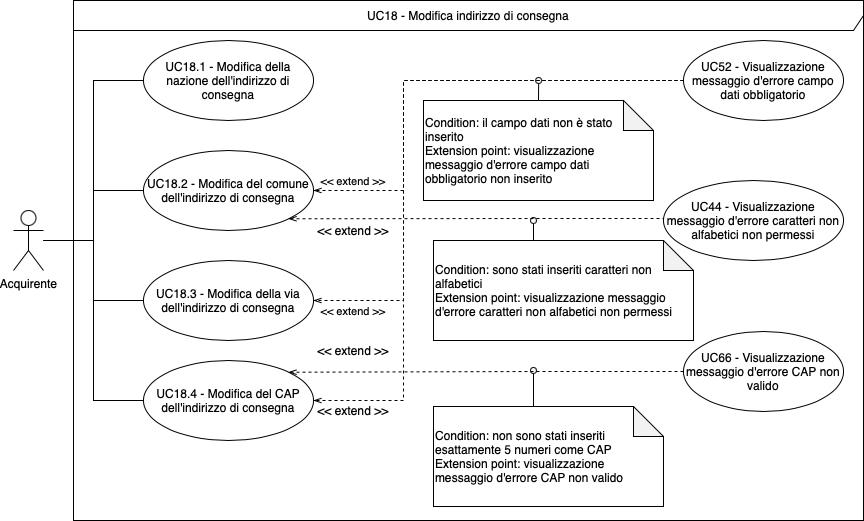
\includegraphics[scale=0.6]{Immagini/DiagrammiUC/Acquirente/ModificaIndirizzoConsegna.png}
    \caption{Diagramma di \actualUC: Modifica indirizzo di consegna} 
    \label{fig:modifica-indirizzo-consegna}
\end{figure}

L'acquirente è nell'operazione di checkout e vuole modificare un indirizzo di consegna precedentemente inserito.
\begin{itemize}
    \item \textbf{Attori primari:} acquirente;
    \item \textbf{Precondizione:} l'acquirente è nell'operazione di checkout e ha selezionato la funzione di modifica di un indirizzo per la consegna precedentemente inserito;
    \item \textbf{Postcondizione:} l'acquirente ha modificato l'indirizzo di consegna desiderata;
    \item \textbf{Scenario principale:} l'acquirente è nell'operazione di checkout e vuole modificare i dati di un indirizzo di consegna precedentemente inserito. Le informazioni che potranno essere modificate sono:
    \begin{itemize}
        \item (UC\ref{modifica-indirizzo-consegna.nazione}) - Modifica della nazione dell'indirizzo di consegna;
		\item (UC\ref{modifica-indirizzo-consegna.comune}) - Modifica del comune dell'indirizzo di consegna;
		\item (UC\ref{modifica-indirizzo-consegna.via}) - Modifica della via dell'indirizzo di consegna;
		\item (UC\ref{modifica-indirizzo-consegna.cap}) - Modifica del CAP dell'indirizzo di consegna.
    \end{itemize}
    In seguito ci sarà la conferma delle modifiche compiute e i dati dell'indirizzo di consegna verranno modificati.
    \item \textbf{Scenari alternativi:}
    \begin{enumerate}[label=\lett]
        \item Se non vengono confermate le modifiche compiute, allora non verranno applicate e andranno perse.
    \end{enumerate}
\end{itemize}

\subUC{Modifica della nazione dell'indirizzo di consegna}
\label{modifica-indirizzo-consegna.nazione}

L'acquirente vuole modificare la nazione dell'indirizzo di consegna.
\begin{itemize}
    \item \textbf{Attori primari:} acquirente;
    \item \textbf{Precondizione:} l'acquirente si trova nella schermata di modifica di un indirizzo di consegna precedentemente inserito;
    \item \textbf{Postcondizione:} l'acquirente ha modificato la nazione dell'indirizzo di consegna;
    \item \textbf{Scenario principale:} l'acquirente modifica correttamente la nazione dell'indirizzo di consegna, selezionandone uno tra quelli disponibili;
    \item \textbf{Scenari alternativi:}
    \begin{enumerate}[label=\lett]
        \item L'acquirente non modifica la nazione dell'indirizzo di consegna attuale e, per questo, non verrà modificato.
    \end{enumerate}
\end{itemize}

\subUC{Modifica del comune dell'indirizzo di consegna}
\label{modifica-indirizzo-consegna.comune}

L'acquirente vuole modificare il comune dell'indirizzo di consegna.
\begin{itemize}
    \item \textbf{Attori primari:} acquirente;
    \item \textbf{Precondizione:} l'acquirente si trova nella schermata di modifica di un indirizzo di consegna precedentemente inserito;
    \item \textbf{Postcondizione:} l'acquirente ha modificato il comune dell'indirizzo di consegna;
    \item \textbf{Scenario principale:} l'acquirente modifica correttamente il comune dell'indirizzo di consegna attraverso le seguenti azioni:
    \begin{itemize}
        \item Si posiziona nel campo dove è presente l'attuale comune dell'indirizzo di consegna;
        \item Modifica il comune dell'indirizzo di consegna.
    \end{itemize}
    \item \textbf{Scenari alternativi:}
    \begin{enumerate}[label=\lett]
        \item L'acquirente non modifica il comune dell'indirizzo di consegna attuale e, per questo, non verrà modificato.
    \end{enumerate}
    \item \textbf{Estensioni:}
    \begin{enumerate}[label=\lett]
        \item L'acquirente elimina l'attuale comune dell'indirizzo di consegna e non ne inserisce uno nuovo. In questo caso:
        \begin{itemize}
            \item (UC\ref{estensione:campo-obbligatorio-non-inserito}) - Viene mostrato il messaggio d'errore campo dati obbligatorio non inserito;
            \item Verrà impedita la modifica dell'indirizzo di consegna.
        \end{itemize}
        \item L'acquirente modifica il comune dell'indirizzo di consegna inserendo dei caratteri non alfabetici. In questo caso:
        \begin{itemize}
            \item (UC\ref{estensione:caratteri-non-alfabetici-non-permessi}) - Viene mostrato il messaggio d'errore caratteri non alfabetici non permessi;
            \item Verrà impedita la modifica dell'indirizzo di consegna.
        \end{itemize}
    \end{enumerate}
\end{itemize}

\subUC{Modifica della via dell'indirizzo di consegna}
\label{modifica-indirizzo-consegna.via}

L'acquirente vuole modificare la via dell'indirizzo di consegna.
\begin{itemize}
    \item \textbf{Attori primari:} acquirente;
    \item \textbf{Precondizione:} l'acquirente si trova nella schermata di modifica di un indirizzo di consegna precedentemente inserito;
    \item \textbf{Postcondizione:} l'acquirente ha modificato la via dell'indirizzo di consegna;
    \item \textbf{Scenario principale:} l'acquirente modifica correttamente la via dell'indirizzo di consegna attraverso le seguenti azioni:
    \begin{itemize}
        \item Si posiziona nel campo dove è presente l'attuale via dell'indirizzo di consegna;
        \item Modifica la via dell'indirizzo di consegna.
    \end{itemize}
    \item \textbf{Scenari alternativi:}
    \begin{enumerate}[label=\lett]
        \item L'acquirente non modifica la via dell'indirizzo di consegna attuale e, per questo, non verrà modificata.
    \end{enumerate}
    \item \textbf{Estensioni:}
    \begin{enumerate}[label=\lett]
        \item L'acquirente elimina l'attuale via dell'indirizzo di consegna e non ne inserisce una nuova. In questo caso:
        \begin{itemize}
            \item (UC\ref{estensione:campo-obbligatorio-non-inserito}) - Viene mostrato il messaggio d'errore campo dati obbligatorio non inserito;
            \item Verrà impedita la modifica dell'indirizzo di consegna.
        \end{itemize}
    \end{enumerate}
\end{itemize}

\subUC{Modifica del CAP dell'indirizzo di consegna}
\label{modifica-indirizzo-consegna.cap}

L'acquirente vuole modificare il CAP dell'indirizzo di consegna.
\begin{itemize}
    \item \textbf{Attori primari:} acquirente;
    \item \textbf{Precondizione:} l'acquirente si trova nella schermata di modifica di un indirizzo di consegna precedentemente inserito;
    \item \textbf{Postcondizione:} l'acquirente ha modificato il CAP dell'indirizzo di consegna;
    \item \textbf{Scenario principale:} l'acquirente modifica correttamente il CAP dell'indirizzo di consegna attraverso le seguenti azioni:
    \begin{itemize}
        \item Si posiziona nel campo dove è presente l'attuale CAP dell'indirizzo di consegna;
        \item Modifica il CAP dell'indirizzo di consegna.
    \end{itemize}
    \item \textbf{Scenari alternativi:}
    \begin{enumerate}[label=\lett]
        \item L'acquirente non modifica il CAP dell'indirizzo di consegna attuale e, per questo, non verrà modificato.
    \end{enumerate}
    \item \textbf{Estensioni:}
    \begin{enumerate}[label=\lett]
        \item L'acquirente elimina l'attuale CAP dell'indirizzo di consegna e non ne inserisce uno nuovo. In questo caso:
        \begin{itemize}
            \item (UC\ref{estensione:campo-obbligatorio-non-inserito}) - Viene mostrato il messaggio d'errore campo dati obbligatorio non inserito;
            \item Verrà impedita la modifica dell'indirizzo di consegna.
        \end{itemize}
        \item L'acquirente modifica il CAP in modo tale che non sia composto da esattamente 5 numeri. In questo caso:
        \begin{itemize}
            \item (UC\ref{estensione:cap-non-valido}) - Viene mostrato il messaggio d'errore CAP non valido;
            \item Verrà impedita la modifica dell'indirizzo di consegna.
        \end{itemize}
    \end{enumerate}
\end{itemize}

%%%%%%%%%%%%%%%%%%%%%%%%%%%%%%%%%%%%%%%%%%%%%%%%%%%%%%%%%%%%%%%%%%%%%%%%%%%%%%%%%%%%%%%%%%%%%%%%%%%%%%%%%%%%%%%%%%%%%%%%%%%%%%%%%%%%%%%%%%%%%%%%%%%%%%%%%%%%%%%%%%%%%%%%%%%%%%

\UC{Eliminazione indirizzo di consegna}
\label{eliminazione-indirizzo-consegna}

L'acquirente vuole eliminare un indirizzo di consegna precedentemente inserito.
\begin{itemize}
    \item \textbf{Attori primari:} acquirente;
    \item \textbf{Precondizione:}  l'acquirente è nell'operazione di checkout;
    \item \textbf{Postcondizione:} l'acquirente ha eliminato l'indirizzo di consegna desiderato.
    \item \textbf{Scenario principale:} l'acquirente è nell'operazione di checkout e vuole eliminare un indirizzo di consegna precedentemente inserito. Per poterlo fare dovrà svolgere le seguenti azioni:
    \begin{itemize}
        \item Seleziona l'indirizzo di consegna da eliminare;
        \item Confermare l'eliminazione della carta.
    \end{itemize}
    Se l'indirizzo di consegna eliminato è quella attualmente selezionato per la consegna e ci sono altri indirizzi di consegna inseriti, allora verrà selezionato per il proseguimento della consegna l'indirizzo successivo. Se viene eliminato l'ultimo indirizzo di consegna e quindi non esiste un indirizzo successivo, verrà selezionato il primo;
    \item \textbf{Scenari alternativi:}
    \begin{enumerate}[label=\lett]
        \item L'acquirente non conferma l'eliminazione dell'indirizzo di consegna e, per questo motivo, non verrà eliminato;
        \item Se l'indirizzo di consegna eliminato dall'acquirente è l'unico attualmente inserito, allora verrà mostrato un messaggio con l'obbligo di dover inserire un nuovo indirizzo di consegna per poter proseguire con il checkout.
    \end{enumerate}
\end{itemize}

%%%%%%%%%%%%%%%%%%%%%%%%%%%%%%%%%%%%%%%%%%%%%%%%%%%%%%%%%%%%%%%%%%%%%%%%%%%%%%%%%%%%%%%%%%%%%%%%%%%%%%%%%%%%%%%%%%%%%%%%%%%%%%%%%%%%%%%%%%%%%%%%%%%%%%%%%%%%%%%%%%%%%%%%%%%%%%